\documentclass{article}
\usepackage[utf8]{inputenc}
\usepackage{array}
\usepackage{multirow}
\usepackage{graphicx}
\usepackage{color}   %May be necessary if you want to color links
\usepackage{hyperref}
\usepackage{longtable}
\usepackage{float}
\usepackage[table]{xcolor}
\setlength{\arrayrulewidth}{0.5mm}
\setlength{\tabcolsep}{18pt}
\renewcommand{\arraystretch}{2.5}
\hypersetup{
    colorlinks=false, %set true if you want colored links
    linktoc=all,     %set to all if you want both sections and subsections linked
    %linkcolor=blue,  %choose some color if you want links to stand out
}

\title{DREAM - RASD}
\author{Filippo Lazzati}
%\date{October 2021}

\begin{document}
\thispagestyle{empty} 
\begin{titlepage}
    \begin{center}
       %\vspace*{2cm}
       {\Huge \textbf{DREAM}} %%Replace this with the Title of your research
       \vspace{0.5cm}
       \\
    \begin{LARGE}
        {Data-dRiven PrEdictive FArMing in Telengana}
        \vspace{1.0cm}
        \\
        {\textit{Requirement Analysis and Specification Document - RASD}}
        
\includegraphics[width=13cm]{logo/polimi.png}
       \vspace{1.5cm}
        
        {Christian Grasso - Filippo Lazzati - Chiara Magri}
       \vspace{0.5cm}
       {Year: 2021/2022}
       
    \end{LARGE}  
   \end{center}
\end{titlepage}
\newpage
\tableofcontents %this command creates an index
\newpage
\section{Introduction}
A RASD\footnote{Requirements Analysis and Specification
Document} is a document that aims to present all the requirements of the system to be developed, explaining the 
domain in which it has to operate. A RASD should work as baseline for the following tasks in software development,
in particular in project planning, software evaluation and change control. Such document has a wide audience, and hence it has to
be written as clear as possible.
\subsection{Purpose}
The main goal that Telengana’s government wants to achieve with \verb|DREAM| is to help policy makers 
formulating policies in the field of agriculture. In order to accomplish this objective, Telengana’s 
government is asking for predictive models for food systems that can drive decisions exploiting huge 
amount of data. Therefore, \verb|DREAM| must be a software system that gather data from some sensors and from the farmers and the agronomists and performs data analysis over it in order to help policy makers doing their job. Moreover, \verb|DREAM| aims to help farmers by putting them in contact with each other so that they can exchange advices and aids. Finally, \verb|DREAM| also schedules the daily work of agronomists and make them visit the worse-performing farmers.
Consequently, the goals of this project are:
\rowcolors{2}{gray!15}{gray!35}
 \begin{longtable}[c]{|m{0.75cm}|m{11cm}|}
%%%%%%%%%%%%%%%%%%%%%%%%%%%%%%%%%%
 \hline
 \multicolumn{2}{|c|}{\cellcolor{white}\textbf{\emph{Goals}}}
 % do not write anything here
 \endfirsthead
 % do not write anything here
 \endhead
 % do not write anything here
 \endfoot
 % do not write anything here
 \endlastfoot
%%%%%%%%%%%%%%%%%%%%%%%%%%%%%%%%%
\hline
G & The policy makers are able to identify best performing farmers, in particular w.r.t resilience toward climatic adverse events, as they will be given incentives and will be asked to provide help to other farmers.\\
  \hline
G & The policy makers are able to identify worst performing farmers, as they need to be receive help for improving their activity.\\
  \hline
G & The policy makers are able to understand if the initiatives involving agronomists and best performing farmers have a good impact on the work of the farmers.\\
  \hline
G & Farmers are able to visualize data weather forecasts regarding their piece of land.\\
  \hline
G & Farmers receive personalized suggestions about crops to plant.\\
  \hline
G & Farmers receive persnalized suggestions about fertilizers to use.\\
  \hline
G & Farmers are able to insert data in the system about their production and any problem they encounter.\\
  \hline
G & Farmers are able to communicate via a forum // discussioni di sicuro non è un goal !!!.\\
  \hline
G & Farmers are able to request for help to agronomists and other farmers.\\
  \hline
G & Agronomists are able to visualize weather forecast for the area they are responsible of.\\
  \hline
G & Agronomists are able to identify the best performing farmers in the area they are responsible of.\\
  \hline
G & Agronomists have a daily plan of visits to farms, where each farm has to be visited at least twice a year, but worst performing farms are visited more often; they can confirm the execution of a plan at the end of the day or specify deviations.\\
  \hline
G & Farmers sono aiutati nella loro produzione e scambiano discussioni.\\
  \hline
  \end{longtable}
\subsection{Scope}

\rowcolors{2}{gray!15}{gray!35}
\begin{longtable}[c]{|m{0.75cm}|m{11cm}|}
%%%%%%%%%%%%%%%%%%%%%%%%%%%%%%%%%%
 \hline
 \multicolumn{2}{|c|}{\cellcolor{white}\textbf{\emph{World phenomena}}}
 % do not write anything here
 \endfirsthead
 % do not write anything here
 \endhead
 % do not write anything here
 \endfoot
 % do not write anything here
 \endlastfoot
%%%%%%%%%%%%%%%%%%%%%%%%%%%%%%%%%
  \hline
 WP1 & In the mandal X, in the day YYYY/MM/DD,  the weather is WW\footnote{sunny | partially cloudy |  cloudy | foggy  |  rainy | stormy | tornado | hurricane}.\\
 \hline
 WP2 & In the mandal X, the maximun, minimum and average temperatures in the day YYYY/MM/DD are TMAX, TMIN and TAVG.\\
 \hline
 WP3 & In the mandal X, the millimeters of rain fallen in the day YYYY/MM/DD are RR.\\
 \hline
 WP4 & In the mandal X, the average wind of the day YYYY/MM/DD has a speed of VV\footnote{N | W | S | E | NW | NE | SE | SW } km/h and a direction DR\\
 \hline
 WP5 & In the mandal X, the average humidity  of the day YYYY/MM/DD  rate is HR.\\
 \hline
 WP6 & In the mandal X, the average atmospheric pressure  of the day YYYY/MM/DD  rate is AP millibars.\\
 \hline
 WP7 & The soil moisture on a terrain T is SM (soil moisture = mass of water/mass of solid particles in the terrain – or volume, depending on the definition).\\
 \hline
 WP8 & A farmers is responsible for a plot of land of area A in the district D.\\
 \hline
 WP9 & A terrain is culivated with (NP plants of) product P.\\
 % not for all products is possible to count the number of plants es cotton -> for there products is sufficient to count the area of the field.
 \hline
 WP10 & A farmer during the day YYYY/MM/DD  plants NS seeds or NP plants of product PR.\\
 \hline
 WP11 & A farmer during the day YYYY/MM/DD  harvests a quantity of K kgs of product PR.\\
 \hline
 WP12 & A farmer during the day YYYY/MM/DD  uses a quantity FQ of fertilizer on a plant P.\\
 \hline
 WP13 &  A farmer waters does manual irrigation on of his fields.\\
 \hline
 WP14 & The water irrigation system  of a terrain TT spreads a quantity WI of water during the day YYYY/MM/DD.\\
 \hline
 WP15 & A farmer faces a problem in his work.\\
 \hline
 WP16 & A farmer is granted an incentive.\\
 \hline
 WP17 & farmer is contacted by a policy maker to take part into initiatives to provide his best practices to others.\\
 \hline
 WP18 & A policy maker is given a password by the Telangana administration.\\
 \hline
 WP19 & An agronomist is responsible for an area A of terrains.\\
 \hline
 WP20 & An agronomist is given a password by the Telangana administration.\\
 \hline
 WP21 & An agronomist visits a farm.\\
 \hline
 \end{longtable}
 
 \rowcolors{2}{gray!15}{gray!35}
 \begin{longtable}[c]{|m{0.75cm}|m{11cm}|}
%%%%%%%%%%%%%%%%%%%%%%%%%%%%%%%%%%
 \hline
 \multicolumn{2}{|c|}{\cellcolor{white}\textbf{\emph{Shared phenomena}}}
 % do not write anything here
 \endfirsthead
 % do not write anything here
 \endhead
 % do not write anything here
 \endfoot
 % do not write anything here
 \endlastfoot
%%%%%%%%%%%%%%%%%%%%%%%%%%%%%%%%%
  \hline
 SP1 & The forecast indicates that in the mandal X, in the day YYYY/MM/DD,  the weather will be WW\footnote{sunny | partially cloudy |  cloudy | foggy  |  rainy | stormy | tornado | hurricane}.\\
 \hline
 SP2 & The forecast indicates that in the mandal X, in  the day | week | month the maximun, minimum and average temperatures will be TMAX, TMIN and TAVG.\\
 \hline
 SP3 & The forecast indicates that in the mandal X, in  the day | week | month the millimeters of rain fallen will be RR.\\
 \hline
 SP4 & The forecast indicates that in the district | mandal X, in  the day | week | month , the average wind will have a speed of VV km/h and a direction DR\footnote{N | W | S | E | NW | NE | SE | SW }.\\
 \hline
 SP5 & The forecast indicates that in the mandal X, in  the day | week | month , the average humidity  rate will be HR.\\
 \hline
 SP6 & The forecast indicates that in the mandal X, in  the day | week | month , the average pressure will be AP millibars.\\
 \hline
 SP7 & The weather reports indicate that in the district | mandal X, in the day YYYY/MM/DD,  the weather was WW\footnote{sunny | partially cloudy |  cloudy | foggy  |  rainy | stormy | tornado | hurricane}.\\
 \hline
 SP8 & The weather reports indicate that in the district | mandal X, in  the day | week | month the maximun, minimum and average temperatures in the day YYYY/MM/DD were TMAX, TMIN and TAVG.\\
 \hline
 SP9 & The weather reports indicate that in the district | mandal X, in  the day | week | month the millimeters of rain fallen in the day YYYY/MM/DD were RR.\\
 \hline
 SP10 & The weather reports indicate that in the district | mandal X, in  the day | week | month , the average wind of the day YYYY/MM/DD had a speed of VV km/h and a direction DR\footnote{N | W | S | E | NW | NE | SE | SW }.\\
 \hline
 SP11 & The weather reports indicate that in the district | mandal X, in  the day | week | month, the average humidity  of the day YYYY/MM/DD  rate were HR.\\
 \hline
 SP12 & •	The weather reports indicate that in district | mandal X, in the day | week | month, the average atmospheric pressure was AP millibars.\\
 \hline
 SP13 & The soil moisture sensor detects a soil moisture on a terrain T of SM\% (soil moisture = mass of water/mass of solid particles in the terrain – or volume, depending on the definition).\\
 \hline
 SP14 & A farmer inserts in DREAMS his personal data (name, surname, contacts).\\
 \hline
 SP15 & A farmers inserts in DREAMS the location and the area of the plot of land that he owns | is responsible of.\\
 \hline
 SP16 & A farmer inserts in DREAMS that in his piece of land, an area A is devoted to the cultivation of product P (and inserts number of plants)  %// not for all products is possible to count the number of plants es cotton -> for there products is sufficient to count the area of the field
 \\
 \hline
 SP17 & A farmes logs in.\\
 \hline
 SP18 & A farmer inserts in DREAMS that during the day YYYY/MM/DD  he has planted NS seeds or NP plants of product PR.\\
 \hline
 SP19 & A farmer inserts in DREAMS that during the day YYYY/MM/DD he has harvested a quantity of K kgs of product PR.\\
 \hline
 SP20 & A farmer inserts in DREAMS during the day YYYY/MM/DD  that he has used a quantity FQ of fertilizer on a plant P.\\
 \hline
 SP21 & The water irrigation system  sensor of a terrain TT measures that a quantity WI of water  has been spread during the day YYYY/MM/DD // we know the location of sensors -> put in DA.\\
 \hline
 SP22 & A farmer inserts in DREAMS that that during the day YYYY/MM/DD he has watered a piece of land PL with a quantity of water WI.\\
 \hline
 SP23 & A farmer visualizes the weather forecasts relative to its land location.\\
 \hline
 SP24 & A farmer visualizes a suggestion regarding a crop to plant in its land.\\
 \hline
 SP25 & A farmer visualizes a suggestion regarding a fertilizer to use.\\
 \hline
 SP26 & A farmer inserts into DREAMS data regarding a problem he has.\\
 \hline
 SP27 & A farmer issues a request for help to an agronomist.\\
 \hline
 SP28 & A farmer issues a request for help to another farmer.\\
 \hline
 SP29 & A farmer responds to a request for help received by another farmer.\\
 \hline
 SP30 & A farmer shares a post on a discussion forum.\\
 \hline
 SP31 & A policy maker inserts his personal data (name, surname, contacts)  into DREAMS when signing up.\\
 \hline
 SP32 & policy maker logs in.\\
 \hline
 SP33 & REAMS shows statistics regarding farmers (type of products, amount produced, fertilizers, watering, location…).\\
 \hline
 SP34 & •	DREAMS shows a list of best performing farmers, considering also resilience towards metereological adverse events.\\
 \hline
 SP35 & •	DREAMS shows a list of worse performing farmers.\\
 \hline
 SP36 & •	DREAMS shows correlations between agronomists and good farmers interventions and farmers statistics // punto da riguardare .\\
 \hline
 SP37 &  policy maker selects a farmer from a list of best performing farmers and saves it as well performing farmer .\\
 \hline
 SP38 & •	A policy maker selects a farmer from a list of worst performing farmers and saves it as badly performing farmer .\\
 \hline
 SP39 & •	An agronomists signs in the DREAMS system.\\
 \hline
 SP40 & •	An agronomist inserts the area A of terrains he is responsible of into the DREAMS system.\\
 \hline
 SP41 & •	An agronomist inserts his personal data (name, surname, contacts) into the DREAMS system.\\
 \hline
 SP42 & •	An agronomist receives a request for help from a farmer.\\
 \hline
 SP43 & •	An agronomist replies to a request for help from a farmer.\\
 \hline
 SP44 & •	An agronomist visualizes the weather forecast for the area he is responsible of.\\
 \hline
 SP & •	An agronomist visualizes a list of the best performing farmers in the area he is responsible of.\\
 \hline
 SP & •	DREAMS computes a daily plan  for an agronomist to visit the farms he is responsible of.\\
 \hline
 SP & •	An agronomist updates his daily plan for visiting farms.\\
 \hline
 SP & •	At the end of a work day, an agronomist confirms the execution of his daily plan for visiting farms.\\
 \hline
 SP & •	At the end of a work day, an agronomist specifies a deviation for his daily plan for visiting farms.\\
 \hline
 SP & •	An agronomist inserts into the system information regarding a visit to a farm.\\
 \hline
 \end{longtable}

\subsection{Definitions, Acronyms, Abbreviations}
\begin{itemize}
    \item WW = sunny | partially cloudy |  cloudy | foggy  |  rainy | stormy | tornado | hurricane
    \item DR = N | W | S | E | NW | NE | SE | SW 
    \item 
\end{itemize}
\subsection{Revision history}
\subsection{Reference Documents}
\subsection{Document Structure}

\section{Overall description}
\subsection{Product perspective}
\subsection{Product functions} \label{Product functions}
In this section, a list of the most important requirements of the system is provided; notice 
that they are just briefly described, since they will be analysed in-depth in chapter 3.
\subsubsection{Data collection}
Just like every data-driven decision, data is essential. \verb |DREAM| must be able to manage different kinds of data coming from different sources:
\begin{enumerate}
\item agronomists and farmers insert into the system standard kind of information about the farms they 
respectively visit and own, but also other kinds of information like, for example, the types of products 
cultivated and the production volume for each product (kinds of information that allow the analytics to 
profile these users). \verb |DREAM| also allows them to insert less-structured data, for instance full-text feedback 
about the inserted data (farmers can insert data about any problem they face);
\item data gathered by sensors deployed on the territory and by the water irrigation system are automatically 
collected by \verb|DREAM| through effective interfaces interacting with such systems;
\item already existing systems are integrated with \verb|DREAM|;
\item the last but not the least, farmers can interact through discussion forums, that are stored by \verb|DREAM|.
\end{enumerate}
\subsubsection{Data analysis}
The raw data collected by \verb|DREAM| must be processed before being delivered to the end-user. Therefore, 
starting with the big volume of information “ingested”, various kinds of analytics are performed in order to 
provide a more aggregate version of the data:
\begin{itemize}
%machine learning techniques are used to customize (for example) the suggestions recommended to the 
%farmers based on their location and their type of production;
\item the suggestions provided to the farmers are customized according to their information;
\item information about farmers’ production is used to distinguish among farmers who are performing well 
and those who are not;% (classification problem);
%data mining algorithms are used to track patterns and identify relations
\item  patterns and relations are identified among the data (for instance between weather 
forecasts and production volumes);
% statistical algorithms are applied for quantifying the improvement (if present) in the crop after having 
% adopted agronomists’ suggestions.
\item analytics are also used for quantifying the improvement (if present) in the crop after having adopted agronomists’ suggestions.
\end{itemize}
\subsubsection{Forum}
As previously mentioned, farmers are allowed to open discussion forums on \verb|DREAM| with other farmers. 
This allows to keep in touch with other people doing the same job and, hence, to ask for advice in case of 
needing.
\subsubsection{Request and supply of help}
There are 4 different ways for a farmer to ask for help: ask for it directly to other farmers, ask in the forum, ask to to
the agronomists or waiting for the system to recognize him as in trouble. As far as the first option is 
concerned, the service is provided through a GUI. On the other side, either farmers who are performing 
well or agronomists may be reached by the system on behalf of other farmers (or of the system itself) for a 
request of help. Then the system introduces them. It should be remarked that a farmer can contact only 
agronomists in the same area.
\subsubsection{Daily plan}
\verb|DREAM| automatically devises a daily plan for each agronomist consisting in a list of farms that must be visited and provides a possible time schedule for such meetings. Every daily plan must be actively accepted 
by the agronomist before the involved farmer is notified. Anyway, the agronomist can apply some changes 
to the schedule, but the system will not approve them if some constraints are violated.
\subsection{User characteristics}
With regards to the possible actors of \verb|DREAM|, three different main user classes can be identified:
\begin{description}
\item \textbf{Policy makers}: their job is to devise policies to regulate the agricultural production. \verb|DREAM| helps 
them providing aggregate data. Policy makers access the system and then receive high-level 
information about which farmers are performing well and which not, and possible reasons to this 
fact. Furthermore, \verb|DREAM| helps to understand the impact of agronomists’ clues in farmers’ 
productions;
\item \textbf{Farmers}: they have a farm and some plots of land to cultivate. They access the system and insert 
data about themselves, helping \verb|DREAM| to profile them. They insert data about their productions, 
the area where they work, eventual problems they must face, questions in the forum … and so on. 
On the other side, \verb|DREAM| puts them in touch with someone who can help them and provides data 
that may be relevant to them;
\item \textbf{Agronomists}: an agronomist has to find methods for increasing the production and the quality of 
the harvest. They insert the area they are responsible of and the they receive data about the best 
performing farmers and weather forecasts. They can answer to farmers’ questions and they receive 
a raw daily plan about which farmers they should visit.
\end{description}
\subsection{Assumptions, dependencies and constraints}

\rowcolors{2}{gray!15}{gray!35}
\begin{longtable}[c]{|m{0.75cm}|m{11cm}|}
%%%%%%%%%%%%%%%%%%%%%%%%%%%%%%%%%%
 \hline
 \multicolumn{2}{|c|}{\cellcolor{white}\textbf{\emph{Domain assumptions}}}
 % do not write anything here
 \endfirsthead
 % do not write anything here
 \endhead
 % do not write anything here
 \endfoot
 % do not write anything here
 \endlastfoot
%%%%%%%%%%%%%%%%%%%%%%%%%%%%%%%%%
  \hline
  D & •	TSDPS (Telengana State Develompent Planning Society) provides weather forecasts and reports, which are available to the DREAMS system // come?.\\
  \hline
  D & •	If the weather reports indicates that in the district | mandal X, in the day YYYY/MM/DD,  the weather was WW,  it was indeed WW.\\
  \hline
  D & •	The maximum, minimum and average temperatures in the weather reports have a precision of TP°C.\\
  \hline
  D & •	The rainfall in the weather reports has a precision of TR mm.\\
  \hline
  D & The wind speed in the weather reports has a precision of WSP km/h.\\
  \hline
  D & The wind direction in the weather reports has a precision of WDP km/h.\\
  \hline
  D & The average humidity in the weather reports has a precision of HP.\\
  \hline
  D & The pressure in the weather reports has a precision of PP millibars.\\
  \hline
  D & Water irrigation system provide data to the DREAMS system in the format , with a precision of WIP /not good.\\
  \hline
  D & Soil moisture sensors are installed  km2 (// balzabile, possiamo anche non assumerlo), and provide data with a precision of SM.\\
  \hline
  D & Each farmer owns a device connected to the Internet network // requirement vago, ma secondo me va bene così.\\
  \hline
  D & Farmers inserts correctly their personal data and data regarding their piece of land.\\
  \hline
  D & Farmers insert correctly data regarding their production (harvest, watering, fertilizers…).\\
  \hline
  D & Rispondono alle richieste di aiuto.\\
  \hline
  D & Opera o su tutto o su nulla (per un certo prodotto).\\
  \hline
  D & Each policy maker owns a personal computer, connected to the Internet network and with a browser installed.\\
  \hline
  D & Policy makers are given a password – associated to their mail – by the Telengana agriculture department.\\
  \hline
  D & Policy makers contact best performing farmers (following an approved protocol established by Telengana government) for granting incentives and asking to collaborate for providing help to other farmers // eliminabile.\\
  \hline
  D & Each agronomist owns a device connected to the Internet network and with a browser installed // oppure un’applicazione mobile? Oppure entrambe?.\\
  \hline
  D & Agronomists are given a password – associated to their mail – by the Telengana agriculture department.\\
  \hline
  D & Agronomists insert correct information regarding their visits to the farms.\\
  \hline
  D & Agronomists reply to help requests issued by farmers.\\
  \hline
  \end{longtable}
\section{Specific requirements}
\subsection{External Interface Requirements}
\subsection{Functional Requirements}
\verb |DREAM| allows its users to perform many tasks, and \verb |DREAM| itself is able to interact with other different systems to achieve some results (see section \ref{Product functions}). In order to provide the main requirements of the system and a summary of the possible situations in which \verb |DREAM| is involved and used, this paragraph first lists all the requirements of the system, then it lists some concrete scenarios \footnote{“A narrative description of what people do and experience as
they try to make use of computer systems and applications” [M.
Carrol, Scenario-based Design, Wiley, 1995]} and finally it abstracts from details and specificities showing the corresponding use cases.
\subsubsection{Requirements}

\rowcolors{2}{gray!15}{gray!35}
\begin{longtable}[c]{|m{0.75cm}|m{11cm}|}
%%%%%%%%%%%%%%%%%%%%%%%%%%%%%%%%%%
 \hline
 \multicolumn{2}{|c|}{\cellcolor{white}\textbf{\emph{Requirements}}}
 % do not write anything here
 \endfirsthead
 % do not write anything here
 \endhead
 % do not write anything here
 \endfoot
 % do not write anything here
 \endlastfoot
%%%%%%%%%%%%%%%%%%%%%%%%%%%%%%%%%
  \hline
  R & The DREAMS system is able to store data regarding users.\\
  \hline
  R & The DREAMS system is able to store data regarding the production of a farmer.\\
  \hline
  R & The DREAMS system is able to store data from the water irrigation system.\\
  \hline
  R & The DREAMS system is able to store data from the soil moisture sensors.\\
  \hline
  R & The DREAMS system is able to store data inserted by agronomists regarding their visit to the farms.\\
  \hline
  R & The DREAMS system is able to compute a list of N best performing farmers (in a certain area A).\\
  \hline
  R & The DREAMS system is able to compute a list of N best performing farmers, also taking into account resilience towards adverse metereological events.\\
  \hline
  R & The DREAMS system is able to compute a list of N worst performing farmers.\\
  \hline
  R & The DREAMS system is able to save the identification of a farmer as well or badly performing farmer done by a policy maker // da esprimere meglio.\\
  \hline
  R & The DREAMS system is able to show statistics about production of farmers.\\
  \hline
  R & The DREAMS system is able to identify possible correlations between improvements in farmers work and activities involving agronomists and best performing farmers.\\
  \hline
  R & The DREAMS system is able to show weather forecasts relative to a certain area.\\
  \hline
  R & The DREAMS system is able to suggest crops to plant to farmers.\\
  \hline
  R & The DREAMS system is able to suggest fertilizers to use to farmers.\\
  \hline
  R & The DREAMS system provides a forum where farmers can discuss.\\
  \hline
  R & The DREAMS system allows a farmer to visualize agronomists available in his area.\\
  \hline
  R & The DREAMS system allows a farmer to request for help to an agronomist in his area.\\
  \hline
  R & The DREAMS system allows an agronomist to reply to a request issued by a farmer.\\
  \hline
  R &  The DREAMS system allows a farmer to visualize best performing farmers.\\
  \hline
  R & The DREAMS system allows a farmer to request for help to a best performing farmer.\\
  \hline
  R & The DREAMS system allows a farmer identified as best performing to reply to a request issued by another farmer.\\
  \hline
  R & The DREAMS system provides agronomists with a daily plan for visiting farms, where each farm in the area assigned to the agronomist is visited at least twice a year.\\
  \hline
  R & The DREAMS system enforces that in the daily plan of agronomists, visits to worst performing farmers are scheduled more often than twice a year.\\
  \hline
  R & The DREAMS system allows agronomists to confirm the execution of the daily plan at the end of the day.\\
  \hline
  R & The DREAMS system allows agronomists to specify deviations from the daily plan at the end of the day.\\
  \hline
  \end{longtable}
\subsubsection{Scenarios}
\paragraph{A storm ruined the harvest}
Arin is a farmer who mainly cultivates potatoes, onions and tomatoes in the fields of his family. The harvest of March was really good, and Arin hoped that the same volume of production might have been repeated in April as well. Unfortunately, the North Indian Ocean cyclone season starts in April, and in the second week of this month Tauktae storm, the strongest storm of of the season, violently hit Arin's lands, halving the crop.\par
\noindent Consequently, Arin wants to share in the system (\verb|DREAM|) the outcome of the storm. Arin opens its browser and access the system using its credentials. Next, he selects from a menu in the incoming webpage the entry for inserting data about production and problems. Then he fills the form with a description about the storm and what it caused to its fields, and finally he sends it.\par
\noindent Arin hopes to receive some aid.
\paragraph{Great year for the potatoes}
Like many other farmers in India, Ikbal knows that the best period for cultivating potatoes is during the months from October to December. The weather is neither hot nor cold and the monsoons are nearly over at this time. Therefore, last October Ikbal planted many potatoes, and in February, with the help of some peasants who work for him, has picked up all of them. \par
\noindent In order to publish in \verb|DREAM| the results of this year potatoes' harvest, he access the system through its computer, opens the form for inserting data about the production and then starts to fill it. The form is quite structured, and requires some data for each entry. After having inserted all the objective information about the crop, Ikbal would like to share something he has found out during this year, namely that planting the potatoes at depth x allows to retrieve substantial crops of this vegetable. Thus, Ikbal fills in also the optional text box and then sends it.
\paragraph{Registering to the system as an agronomist}
Dalbir worked for many years as an agronomist in Bihar, but recently he has been moved to Telengana. Telengana uses this innovative system, \verb|DREAM|, to keep track of the harvests of farmers, to collect interesting data from sensors and many other things. All the agronomists in Telengana must work with \verb|DREAM|, therefore Dalbir has to create an account. \par
\noindent Dalbir opens the webpage of \verb|DREAM| and initiates the procedure for creating a new account. He follows the procedure tailored for agronomists, which allows him to create a new username and password. Next, Dalbir has to insert some data about his job in order to finish the registration. Among the others, Dalbir is asked to insert the area where he works.\par
\noindent His data will be verified later.
\paragraph{Visiting a farm}
The first task of Dalbir is to visit the farm of Arin. The date and hour of the meeting has been established by \verb |DREAM|, which has notified also Arin about the meeting. Arin has been chosen because last month he performed very bad.\par
\noindent During the meeting, Arin has the opportunity of explaining all the problems he faced during the past month, one for all Tauktae (the strongest storm of the North Indian Ocean cyclone season). Arin takes Dalbir to the fields, where Dalbir can gather some sample from the terrain. At the end of the meeting, Dalbir gives Arin some advices, and then he moves to another farm. \par
\noindent Once in the office, Dalbir inserts in the system a report about his visit to Arin's farm.
\paragraph{A bad schedule}
Like every evening, Dalbir accesses \verb|DREAM| for downloading the daily plan of the next day. Every daily plan provided by the system contains time and place of every meeting, in addition to some information about the farmer. Dalbir notices that Ikbal's farm is closer to his parents' house, and Dalbir knows that they would be really happy to if he had lunch with them.\par
\noindent However, the meeting with Ikbal is scheduled for the 3p.m o' clock. Therefore, Dalbir decides to exchange the meetings with Ikbal and Tarak, visiting Ikbal at 11.30a.m. and Tarak at 3p.m.. Through the user interface of \verb|DREAM|, Dalbir exhanges the two meetings and once he has confirmed, \verb|DREAM| notifies the farmers of the change.
%\paragraph{Collecting data(?)}
% \verb|DREAM| is a software system designed to provide various kinds of analytics to its users, in particular to the policy makers. As a matter of fact, policy makers want to distinguish between well- and bad- performing farmers, as well as understand the impact of initiatives carried out by the agronomists and find patterns and relations among the data.\par
\noindent Therefore, periodically, \verb|DREAM| interacts with sensors deployed on the territory in order to retrieve the humidity of the soil, with the water irrigation system to retrieve the amount of water used by each farmer and with an already existing website which provides up-to-date weather forecasts. In particular:
\begin{itemize}
    \item 3 times a day the soil sensors are asked to provide data about the humidity of the soil;
    \item once a day the water irrigation system is asked to provide the water used by each farmer (when the data is available);
    \item the weather forecasts website is accessed monthly to compute some analytics on the data, but also on demand when agronomists or farmers ask for weather forecasts.
\end{itemize}

\subsubsection{Use cases}
%\paragraph{Use case 1 - InsertProblems}
%\begin{center} %leave it to start the table at newline

\rowcolors{2}{blue!15}{blue!25}
\begin{longtable}{|p{3.5cm}|m{8cm}|}
 \hline
 \multicolumn{2}{|c|}{\cellcolor{white}\emph{USE CASE 1}} \\
 % do not write anything here
 \endfirsthead
 % do not write anything here
 \endhead
 % do not write anything here
 \endfoot
 % do not write anything here
 \endlastfoot
 \hline
 Name & InsertProblems\\
 \hline
 Actor & Farmer\\
 \hline
 Entry condition & The farmer faces a problem and decides to communicate it on \verb|DREAM|\\
 \hline
 Event flow & \begin{enumerate}
    \item The farmer accesses the system through its username and password;
    \item in the homepage, the farmer selects from the menu the item "insert problem";
    \item the farmer selects the kind of problem, when it occurred and how much it lasted;
    \item the farmer gives a brief description of the problem;
    \item the farmer selects whether he likes to meet as soon as possible an agronomist;
    \item the farmer clicks on the "send" button;
    \item \verb|DREAM| automatically detects where is the farm from the account of the farmer;
    \item \verb|DREAM| stores the data and eventually takes into account the request of a meeting with an agronomist.
 \end{enumerate}\\
 \hline
 Exit condition & The problem is saved in the \verb|DREAM| database and, if requested, an agronomist is scheduled to meet the farmer in the next days. The farmer is notified about the meeting.\\
 \hline
 Exceptions & \begin{itemize}
     \item If the kind of problem is not present, the farmer can add it by its own.
     \item In case no agronomist can be scheduled for the current week, the farmer is notified about the problem and an agronomist will be found for the next week.
 \end{itemize}\\
 \hline
 Special requirements & \begin{itemize}
     \item The availability of an agronomist is checked in less than 3 second;
     \item the page is refreshed in less than 1 second.
 \end{itemize}\\
 \hline
\end{longtable}
\begin{figure}[H]
    \centering
    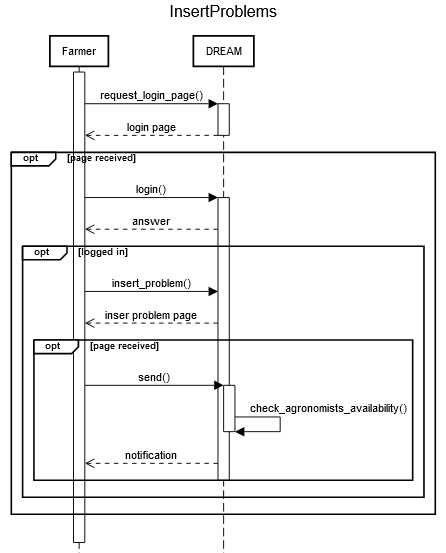
\includegraphics[scale=0.75]{sequence_diagrams/InsertProblems}
    \caption{Sequence diagram for the InsertProblems use case}
\end{figure}
%%%%%%%%%%%TABLE 2%%%%%%%%%%%%%%%%%%%%%%%%%%%%%%%%%%%%%%%%

\centering
\begin{longtable}{|p{3.5cm}|m{8cm}|}
 \hline
 \multicolumn{2}{|c|}{\cellcolor{white}\emph{USE CASE 2}} \\
  % do not write anything here
 \endfirsthead
 % do not write anything here
 \endhead
 % do not write anything here
 \endfoot
 % do not write anything here
 \endlastfoot
 \hline
 Name & InsertProductions\\
 \hline
 Actor & Farmer\\
 \hline
 Entry condition & The farmer gets the results of a crop\\
 \hline
 Event flow & \begin{enumerate}
    \item The farmer accesses the system through its username and password;
    \item in the homepage, the farmer selects from the menu the item "insert productions";
    \item the farmer inserts the picked product, when it was planted, the volume planted, the volume picked;
    \item the farmer optionally gives a brief description of the harvest or an observation he made;
    \item the farmer clicks on the "send" button;
    \item \verb|DREAM| automatically detects where is the farm from the account of the farmer;
    \item \verb|DREAM| stores the data.
 \end{enumerate}\\
 \hline
 Exit condition & The data is saved in the \verb|DREAM| database and the farmer is notified.\\
 \hline
 Exceptions & \begin{itemize}
     \item If the kind of product is not present, the farmer can add it by its own.
 \end{itemize}\\
 \hline
 Special requirements & \begin{itemize}
     \item the page is refreshed in less than 1 second.
 \end{itemize}\\
 \hline
\end{longtable}

\begin{figure}[H]
    \centering
    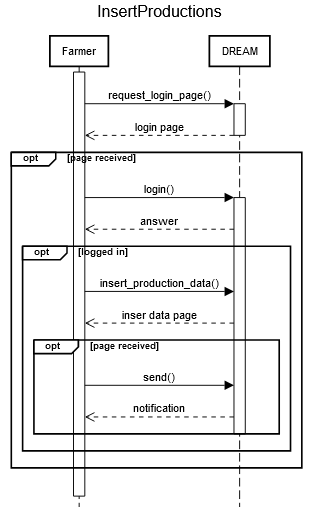
\includegraphics[scale=0.75]{sequence_diagrams/InsertProductions}
    \caption{Sequence diagram for the InsertProductions use case}
\end{figure}
%%%%%%%%%%%%%%%%%%%%%%%%%%%%TABLE 3%%%%%%%%%%%%%%%%%%%%%%%

\centering
\begin{longtable}{|p{3.5cm}|m{8cm}|}
 \hline
 \multicolumn{2}{|c|}{\cellcolor{white}\emph{USE CASE 3}} \\
  % do not write anything here
 \endfirsthead
 % do not write anything here
 \endhead
 % do not write anything here
 \endfoot
 % do not write anything here
 \endlastfoot
 \hline
 Name & RegisterAgronomist\\
 \hline
 Actor & Agronomist\\
 \hline
 Entry condition & The agronomist does not have an account.\\
 \hline
 Event flow & \begin{enumerate}
    \item The agronomist goes to the \verb|DREAM| homepage;
    \item the agronomist selects "create account", then "create agronomist account";
    \item the agronomist inserts his e-mail and devises a password;
    \item the system verifies the e-mail of the agronomist;
    \item the agronomist inserts personal data like name, surname, date of birth, specialization;
    \item the agronomist selects the area where he will work;
    \item the agronomist clicks on "done";
    \item \verb|DREAM| verifies the identity of the agronomist;
    \item the agronomist is notified that he can begin to work.
 \end{enumerate}\\
 \hline
 Exit condition & The agronomist's account is saved in the \verb|DREAM| database and the identity of the agronomist has been verified.\\
 \hline
 Exceptions & \begin{itemize}
     \item If the e-mail is already used, the agronomist is forced to change it;
     \item If the password is too short, the agronomist is forced to change it;
     \item if the identity of the agronomist cannot be verified, a mail notifying the error is sent to the agronomist.
 \end{itemize}\\
 \hline
 Special requirements & \begin{itemize}
     \item the identity must be verified within 3 days.
 \end{itemize}\\
 \hline
\end{longtable}

\begin{figure}[H]
    \centering
    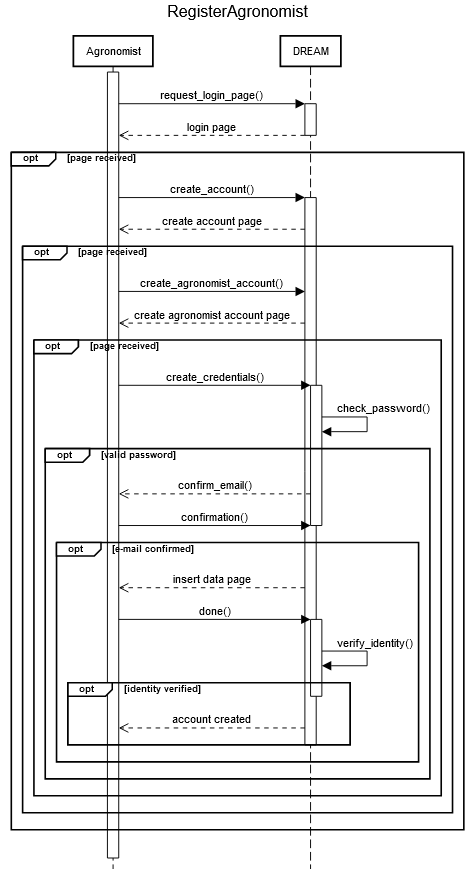
\includegraphics[scale=0.60]{sequence_diagrams/RegisterAgronomist}
    \caption{Sequence diagram for the RegisterAgronomist use case}
\end{figure}
%%%%%%%%%%%%%%%%%%%%%%%%%%%%TABLE 4%%%%%%%%%%%%%%%%%%%%%%%

\centering
\begin{longtable}{|p{3.5cm}|m{8cm}|}
 \hline
 \multicolumn{2}{|c|}{\cellcolor{white}\emph{USE CASE 4}} \\
  % do not write anything here
 \endfirsthead
 % do not write anything here
 \endhead
 % do not write anything here
 \endfoot
 % do not write anything here
 \endlastfoot
 \hline
 Name & RegisterFarmer\\
 \hline
 Actor & Farmer\\
 \hline
 Entry condition & The farmer does not have an account.\\
 \hline
 Event flow & \begin{enumerate}
    \item The farmer goes to the \verb|DREAM| homepage;
    \item the farmer selects "create account", then "create farmer account";
    \item the farmer inserts his e-mail and devises a password;
    \item the system verifies the e-mail of the farmer;
    \item the farmer inserts personal data like name, surname, date of birth, location of the farm;
    \item the farmer clicks on "done";
    \item the farmer is notified that the account has been created.
 \end{enumerate}\\
 \hline
 Exit condition & The farmer's account is saved in the \verb|DREAM| database and the existence of the farm has been verified.\\
 \hline
 Exceptions & \begin{itemize}
     \item If the e-mail is already used, the farmer is forced to change it;
     \item If the password is too short, the farmer is forced to change it.
 \end{itemize}\\
 \hline
 Special requirements & \begin{itemize} 
 \end{itemize}\\
 \hline
\end{longtable}

\begin{figure}[H]
    \centering
    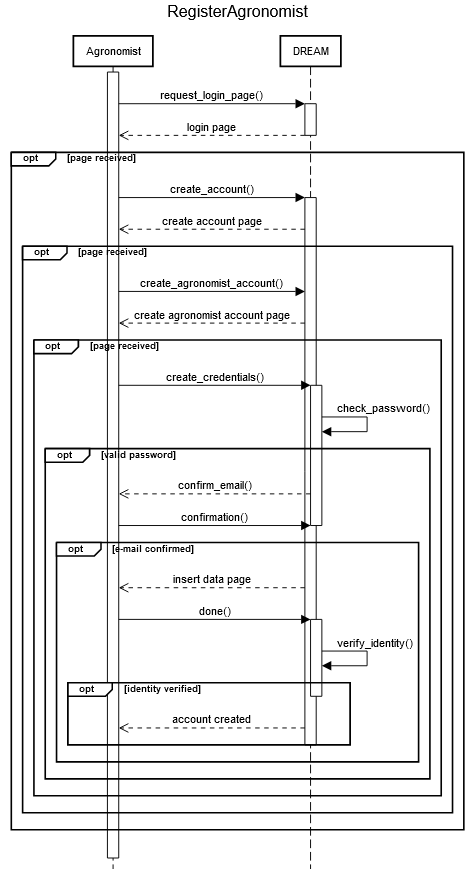
\includegraphics[scale=0.60]{sequence_diagrams/RegisterAgronomist}
    \caption{Sequence diagram for the RegisterFarmer use case}
\end{figure}



%%%%%%%%%%%%%%%%%%%%%%%%%%%%TABLE 5%%%%%%%%%%%%%%%%%%%%%%%

\centering
\begin{longtable}{|p{3.5cm}|m{8cm}|}
 \hline
 \multicolumn{2}{|c|}{\cellcolor{white}\emph{USE CASE 5}} \\
  % do not write anything here
 \endfirsthead
 % do not write anything here
 \endhead
 % do not write anything here
 \endfoot
 % do not write anything here
 \endlastfoot
 \hline
 Name & VisitFarm\\
 \hline
 Actor & Agronomist, Farmer\\
 \hline
 Entry condition & The agronomist is scheduled to visit a farm. The farmer and the agronomist have been informed of the meeting. The time of the meeting occurs.\\
 \hline
 Event flow & \begin{enumerate}
    \item The agronomist is scheduled to visit a certain farm at a certain time;
    \item the farmer is notified about the meeting;
    \item the agronomist accesses \verb|DREAM|;
    \item the agronomist selects "insert farm data";
    \item the agronomist selects the farm and inserts data with a comment;
    \item the agronomist clicks on "done";
    \item \verb|DREAM| stores the data.
 \end{enumerate}\\
 \hline
 Exit condition & The data about the meeting has been inserted by the agronomist and stored in \verb|DREAM|.
 \hline
 Exceptions & \begin{itemize}
     \item If the farmer does not show up at the meeting, the agronomist specifies so when inserting data about the meeting.
 \end{itemize}\\
 \hline
 Special requirements & None\\
 \hline
\end{longtable}


\begin{figure}[H]
    \centering
    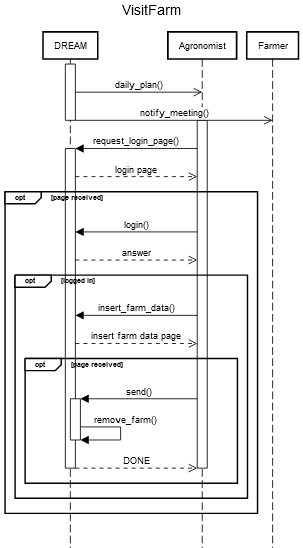
\includegraphics[scale=0.75]{sequence_diagrams/VisitFarm}
    \caption{Sequence diagram for the VisitFarm use case}
\end{figure}
%%%%%%%%%%%%%%%%%%%%%%%%%%%%TABLE 6%%%%%%%%%%%%%%%%%%%%%%%

\centering
\begin{longtable}{|p{3.5cm}|m{8cm}|}
 \hline
 \multicolumn{2}{|c|}{\cellcolor{white}\emph{USE CASE 6}} \\
  % do not write anything here
 \endfirsthead
 % do not write anything here
 \endhead
 % do not write anything here
 \endfoot
 % do not write anything here
 \endlastfoot
 \hline
 Name & GenerateDailyPlan\\
 \hline
 Actor & Agronomist, Farmer\\
 \hline
 Entry condition & The next day is a working day and the agronomist accesses the system.\\
 \hline
 Event flow & \begin{enumerate}
    \item The agronomist receives a daily plan for the following day;
    \item if it is ok for the agronomist, he clicks on  "accept", otherwise he clicks on "change it";
    \item the agronomist selects some changes, then he clicks on "accept";
    \item \verb|DREAM| checks if the new daily plan is acceptable;
    \item the farmer is notified about the meeting.
 \end{enumerate}\\
 \hline
 Exit condition & The daily plan has been confirmed and the farmer has been notified.\\
 \hline
 Exceptions & \begin{itemize}
     \item In case the agronomist does not accept the daily plan, the farmers are not notified about the meeting;
     \item if the daily plan is not acceptable, an error is notified to the agronomist, who has to re-accept (or re-change) the schedule until \verb|DREAM| accepts it;
 \end{itemize}\\
 \hline
 Special requirements &\begin{itemize}
     \item Every farmer must be visited at least twice a year;
     \item bad performing farmers must be visited more times than the others.
 \end{itemize}\\
 \hline
\end{longtable}
\begin{figure}[H]
    \centering
    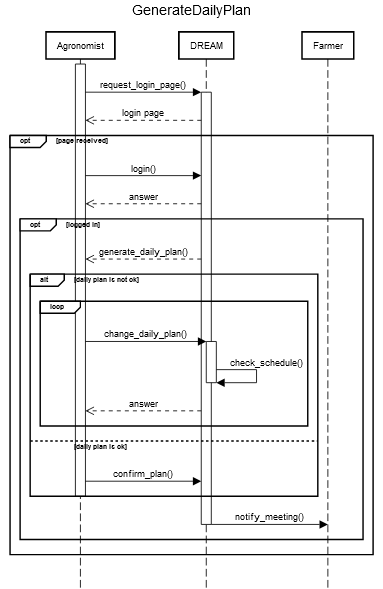
\includegraphics[scale=0.75]{sequence_diagrams/GenerateDailyPlan}
    \caption{Sequence diagram for the GenerateDailyPlan use case}
\end{figure}


%%%%%%%%%%%%%%%%%%%%%%%%%%%%TABLE 7%%%%%%%%%%%%%%%%%%%%%%%

\centering
\begin{longtable}{|p{3.5cm}|m{8cm}|}
 \hline
 \multicolumn{2}{|c|}{\cellcolor{white}\emph{USE CASE 7}} \\
  % do not write anything here
 \endfirsthead
 % do not write anything here
 \endhead
 % do not write anything here
 \endfoot
 % do not write anything here
 \endlastfoot
 \hline
 Name & GetSoilSensorsData\\
 \hline
 Actor & SoilSensors\\
 \hline
 Entry condition & A timer has expired.\\
 \hline
 Event flow & \begin{enumerate}
    \item \verb|DREAM| asks the soil sensors for some data;
    \item the soil sensors answer with the data;
    \item \verb|DREAM| stores the data in its database.
 \end{enumerate}\\
 \hline
 Exit condition & \verb|DREAM| has stored in its database the data coming from the sensors.\\
 \hline
 Exceptions & \begin{itemize}
     \item In case a sensor is not reachable, \verb|DREAM| stores that the data of that sensor at that time is not available because "the sensor is not reachable".
 \end{itemize}\\
 \hline
 Special requirements &\begin{itemize}
     \item The sensor must answer in less than 5 seconds;
     \item \verb|DREAM| must try to contact the sensor 3 times before giving up.
 \end{itemize}\\
 \hline
\end{longtable}
\begin{figure}[H]
    \centering
    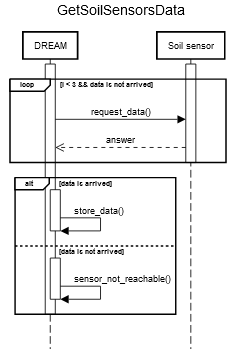
\includegraphics[scale=0.75]{sequence_diagrams/GetSoilSensorsData}
    \caption{Sequence diagram for the GetSoilSensorsData use case}
\end{figure}


%%%%%%%%%%%%%%%%%%%%%%%%%%%%TABLE 8%%%%%%%%%%%%%%%%%%%%%%%

\centering
\begin{longtable}{|p{3.5cm}|m{8cm}|}
 \hline
 \multicolumn{2}{|c|}{\cellcolor{white}\emph{USE CASE 8}} \\
  % do not write anything here
 \endfirsthead
 % do not write anything here
 \endhead
 % do not write anything here
 \endfoot
 % do not write anything here
 \endlastfoot
 \hline
 Name & GetWaterIrrigationSystemData\\
 \hline
 Actor & WaterIrrigationSystem\\
 \hline
 Entry condition & A timer has expired.\\
 \hline
 Event flow & \begin{enumerate}
    \item \verb|DREAM| asks the water irrigation system for some data;
    \item the water irrigation system answers with the data;
    \item \verb|DREAM| stores the data in its database.
 \end{enumerate}\\
 \hline
 Exit condition & \verb|DREAM| has stored in its database the data coming from the water irrigation system.\\
 \hline
 Exceptions & \begin{itemize}
     \item In case the water irrigation system is not reachable, \verb|DREAM| stores that the data of the water irrigation system at that time is not available because "the water irrigation system is not reachable".
 \end{itemize}\\
 \hline
 Special requirements &\begin{itemize}
     \item The water irrigation system must answer in less than 5 seconds;
     \item \verb|DREAM| must try to contact the sensor 3 times before giving up.
 \end{itemize}\\
 \hline
\end{longtable}
\begin{figure}[H]
    \centering
    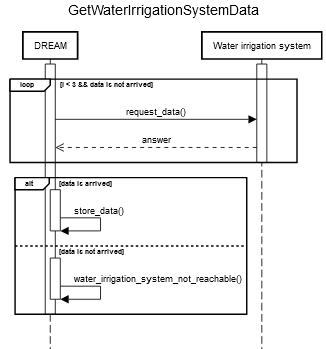
\includegraphics[scale=0.75]{sequence_diagrams/GetWaterIrrigationSystemData}
    \caption{Sequence diagram for the GetWaterIrrigationSystemData use case}
\end{figure}


%%%%%%%%%%%%%%%%%%%%%%%%%%%%TABLE 9%%%%%%%%%%%%%%%%%%%%%%%

\centering
\begin{longtable}{|p{3.5cm}|m{8cm}|}
 \hline
 \multicolumn{2}{|c|}{\cellcolor{white}\emph{USE CASE 9}} \\
  % do not write anything here
 \endfirsthead
 % do not write anything here
 \endhead
 % do not write anything here
 \endfoot
 % do not write anything here
 \endlastfoot
 \hline
 Name & VisualizeAggregateData\\
 \hline
 Actor & PolicyMaker\\
 \hline
 Entry condition & A policy maker accesses the platform and enters the \emph{Aggregate Data} section.\\
 \hline
 Event flow & \begin{enumerate}
    \item The policy maker accesses the system;
    \item the policy maker selects the \emph{Aggregate Data} menu item;
    \item the policy maker chooses the date range they wish to analyze;
    \item \verb|DREAM| generates aggregate statistics for all areas in the database;
    \item \verb|DREAM| shows the data to the user.
 \end{enumerate}\\
 \hline
 Exit condition & The user finishes analyzing the data.\\
 \hline
 Exceptions & \begin{itemize}
     \item If the system has not yet collected any data for the specified period, a warning is returned.
 \end{itemize}\\
 \hline
 Special requirements &\begin{itemize}
     \item The data generation must be completed in less than 3 seconds.
 \end{itemize}\\
 \hline
\end{longtable}

\begin{figure}[H]
    \centering
	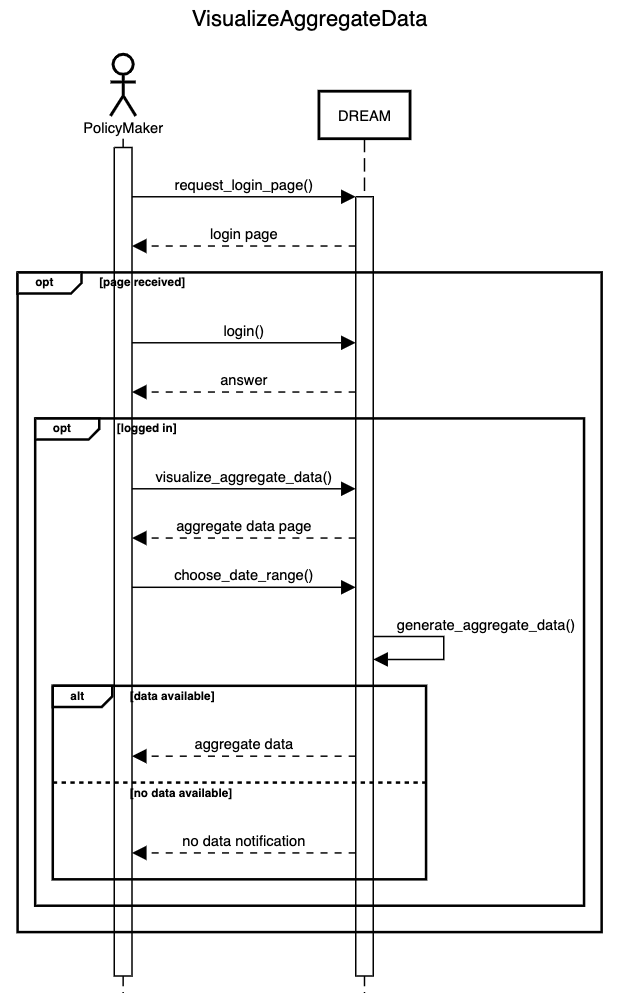
\includegraphics[scale=0.5]{sequence_diagrams/VisualizeAggregateData}
    \caption{Sequence diagram for the VisualizeAggregateData use case}
\end{figure}


%%%%%%%%%%%%%%%%%%%%%%%%%%%%TABLE 10%%%%%%%%%%%%%%%%%%%%%%%

\centering
\begin{longtable}{|p{3.5cm}|m{8cm}|}
 \hline
 \multicolumn{2}{|c|}{\cellcolor{white}\emph{USE CASE 10}} \\
  % do not write anything here
 \endfirsthead
 % do not write anything here
 \endhead
 % do not write anything here
 \endfoot
 % do not write anything here
 \endlastfoot
 \hline
 Name & VisualizeBestFarmers\\
 \hline
 Actor & Agronomist\\
 \hline
 Entry condition & An agronomist accesses the platform and enters the \emph{Farms} section.\\
 \hline
 Event flow & \begin{enumerate}
    \item The agronomist accesses the system;
    \item the agronomist selects the \emph{Farms} menu item;
    \item optionally, the agronomist chooses how the farms should be ranked (e.g. most productive, most resilient to bad weather, ...);
    \item \verb|DREAM| shows a list of the best farms ordered according to the selected parameter.
 \end{enumerate}\\
 \hline
 Exit condition & The user finishes analyzing the data.\\
 \hline
 Exceptions & \begin{itemize}
     \item If the system has not yet collected any data in the agronomist's area, a warning is shown.
 \end{itemize}\\
 \hline
 Special requirements &\begin{itemize}
     \item The data must be shown in less than 1 second.
 \end{itemize}\\
 \hline
\end{longtable}

\begin{figure}[H]
    \centering
	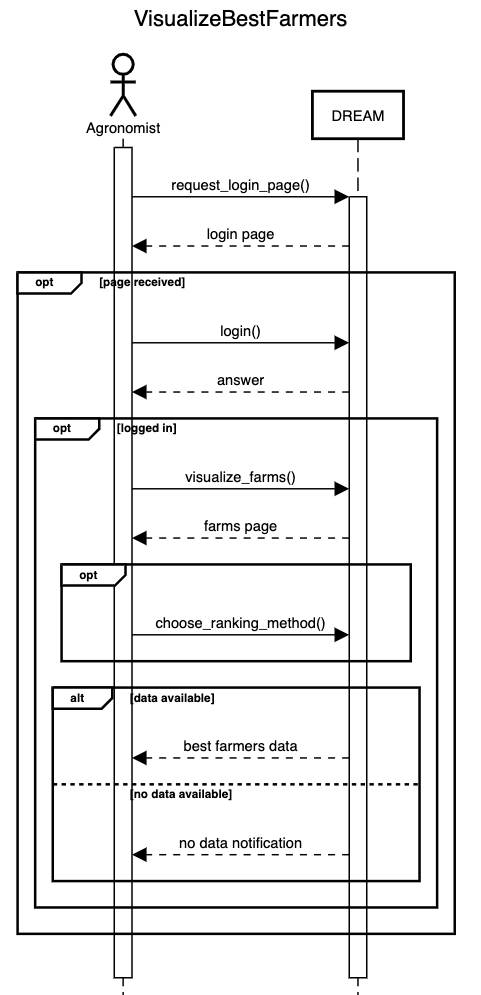
\includegraphics[scale=0.5]{sequence_diagrams/VisualizeBestFarmers}
    \caption{Sequence diagram for the VisualizeBestFarmers use case}
\end{figure}

%%%%%%%%%%%%%%%%%%%%%%%%%%%%TABLE 11%%%%%%%%%%%%%%%%%%%%%%%

\centering
\begin{longtable}{|p{3.5cm}|m{8cm}|}
 \hline
 \multicolumn{2}{|c|}{\cellcolor{white}\emph{USE CASE 11}} \\
  % do not write anything here
 \endfirsthead
 % do not write anything here
 \endhead
 % do not write anything here
 \endfoot
 % do not write anything here
 \endlastfoot
 \hline
 Name & VisualizeForecasts\\
 \hline
 Actor & Agronomist\\
 \hline
 Entry condition & An agronomist accesses the platform and enters the \emph{Weather Forecasts} section.\\
 \hline
 Event flow & \begin{enumerate}
    \item The agronomist accesses the system;
    \item the agronomist selects the \emph{Weather Forecasts} menu item;
    \item the agronomist chooses the date for which forecasts should be shown;
    \item \verb|DREAM| connects to the Telengana government website to fetch forecasts for the chosen date;
    \item \verb|DREAM| shows a map with the forecast.
 \end{enumerate}\\
 \hline
 Exit condition & The user finishes analyzing the data.\\
 \hline
 Exceptions & \begin{itemize}
     \item If the Telengana government website is currently unreachable, an error is shown to the user.
     \item If no weather data is available for the chosen date, an error is shown to the user.
 \end{itemize}\\
 \hline
 Special requirements &\begin{itemize}
     \item The Telengana government website must serve requests in less than 5 seconds;
     \item The Telengana government website is assumed not to change in a backwards-incompatible manner without notice.
 \end{itemize}\\
 \hline
\end{longtable}

\begin{figure}[H]
    \centering
	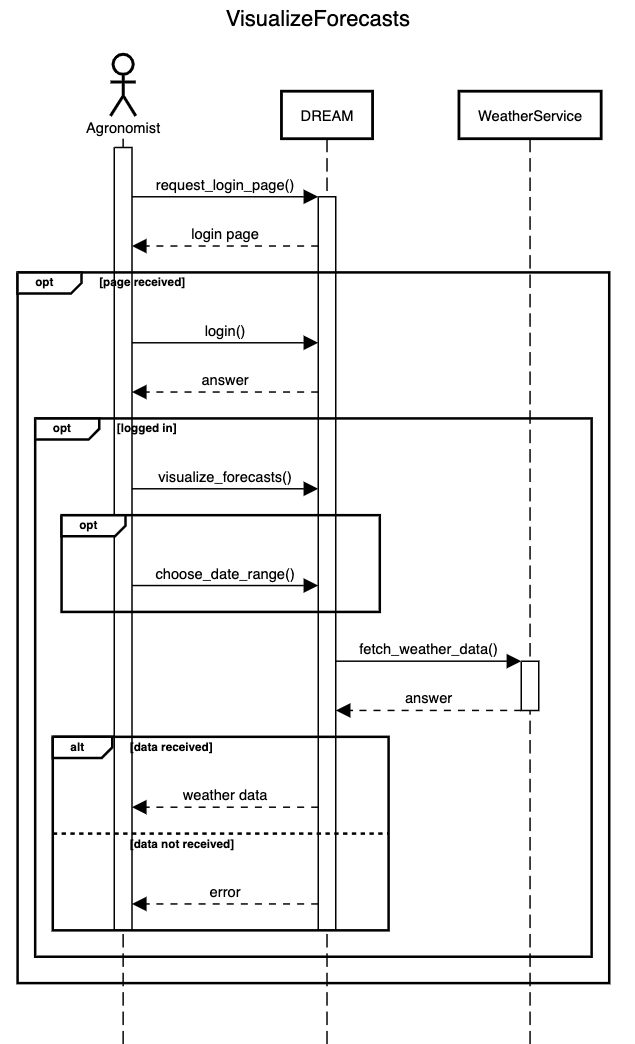
\includegraphics[scale=0.5]{sequence_diagrams/VisualizeForecasts}
    \caption{Sequence diagram for the VisualizeForecasts use case}
\end{figure}
%%%%%%%%%%%%%%%%%%%%%%%%%%%%TABLE 12%%%%%%%%%%%%%%%%%%%%%%%

\centering
\begin{longtable}{|p{3.5cm}|m{8cm}|}
 \hline
 \multicolumn{2}{|c|}{\cellcolor{white}\emph{USE CASE 12}} \\
  % do not write anything here
 \endfirsthead
 % do not write anything here
 \endhead
 % do not write anything here
 \endfoot
 % do not write anything here
 \endlastfoot
 \hline
 Name & VisualizeFarmerSuggestions\\
 \hline
 Actor & Farmer\\
 \hline
 Entry condition & A farmer wants to check if there are any suggestions for them.\\
 \hline
 Event flow & \begin{enumerate}
    \item The farmer accesses the system;
    \item the farmer accesses the \emph{Suggestions} section;
    \item \verb|DREAM| automatically shows suggestions for the farmer.
 \end{enumerate}\\
 \hline
 Exit condition & The farmer views the list of suggestions.\\
 \hline
 Exceptions & \begin{itemize}
     \item If there are no suggestions for the farmer, a notice is shown.
 \end{itemize}\\
 \hline
 Special requirements & None.\\
 \hline
\end{longtable}
\newpage
%%%%%%%%%%%%%%%%%%%%%%%%%%%%TABLE 13%%%%%%%%%%%%%%%%%%%%%%%

\centering
\begin{longtable}{|p{3.5cm}|m{8cm}|}
 \hline
 \multicolumn{2}{|c|}{\cellcolor{white}\emph{USE CASE 13}} \\
  % do not write anything here
 \endfirsthead
 % do not write anything here
 \endhead
 % do not write anything here
 \endfoot
 % do not write anything here
 \endlastfoot
 \hline
 Name & GetWeatherForecasts\\
 \hline
 Actor & OuterWeatherSource\\
 \hline
 Entry condition & Either (a) a user requests weather data; or (b) \verb|DREAM| needs to access weather information for statistical purposes.\\
 \hline
 Event flow & \begin{enumerate}
    \item \verb|DREAM| connects to the Telengana government website to fetch the required forecasts;
    \item The data is stored and analyzed as needed.
 \end{enumerate}\\
 \hline
 Exit condition & The weather forecast data is collected by the system.\\
 \hline
 Exceptions & \begin{itemize}
     \item If the Telengana government website is currently unreachable, the process is aborted and an error is returned.
 \end{itemize}\\
 \hline
 Special requirements &\begin{itemize}
     \item The Telengana government website must serve requests in less than 5 seconds;
     \item The Telengana government website is assumed not to change in a backwards-incompatible manner without notice.
 \end{itemize}\\
 \hline
\end{longtable}
\newpage
\raggedright
\subsection{Performance Requirements}
\subsection{Design Constraints}
\subsection{Software System Attributes}
\section{Formal analysis using Alloy}
\section{Effort spent}
\section{References}
\end{document}
